\section{Abbilden - ER zu Relational}
\label{sec:abbilden}

\begin{figure}[H]\centering\label{Abbilden}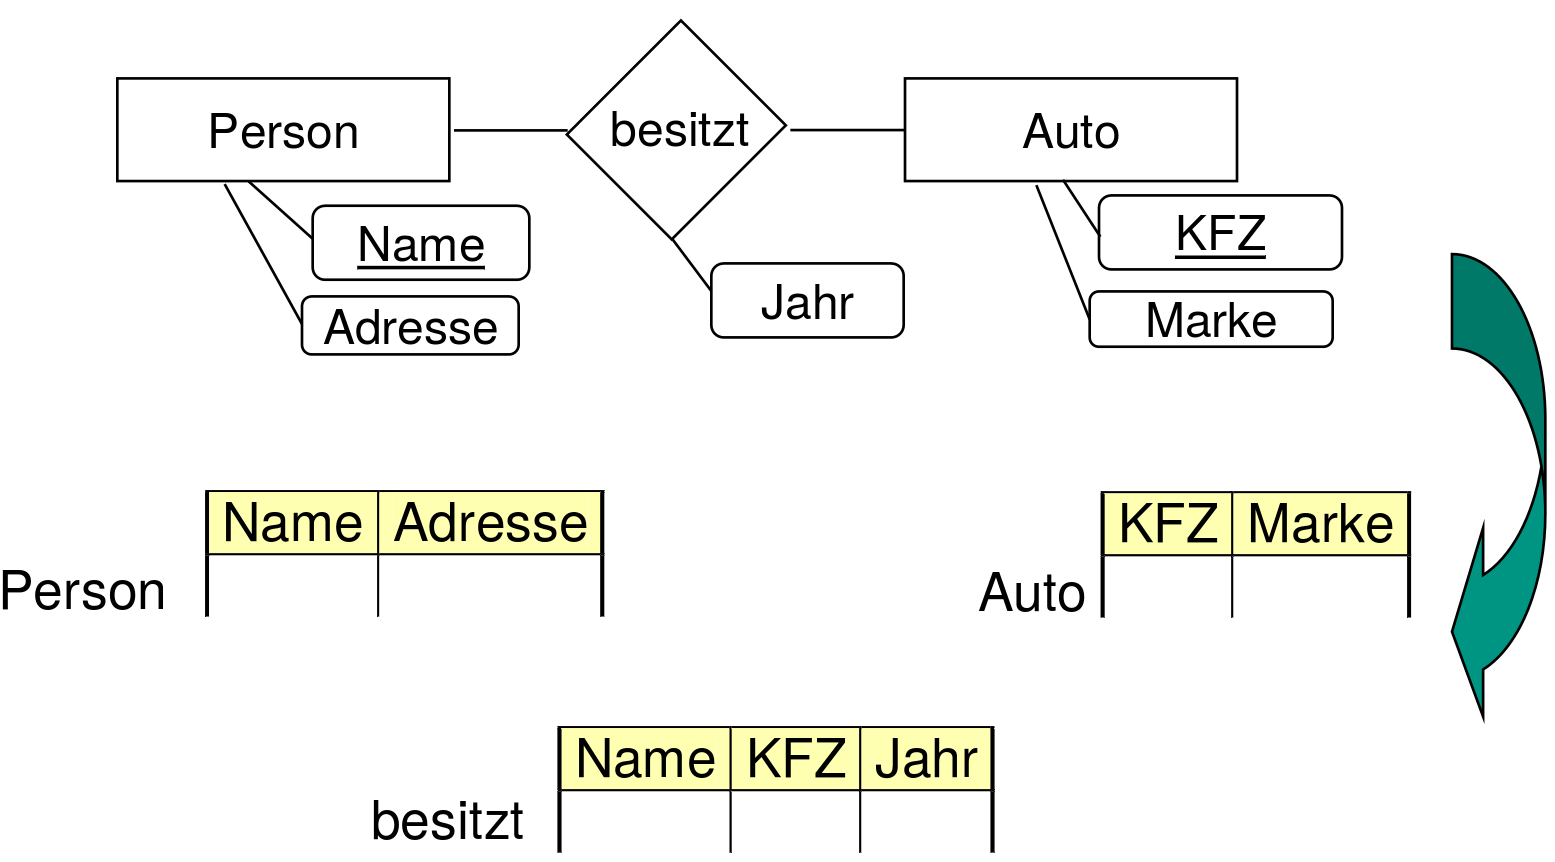
\includegraphics[width=0.33\textwidth]{Abbilden}\end{figure}

\textbf{Abbildungsziel: Kapazitätserhaltende Abbildung}
\begin{items}
	\item In beiden Fällen gleich viele Instanzen darstellbar
	\item \underline{Zu Vermeiden:}
	\item Kapazitätserhöhend: relational mehr darstellbar als mit ER
	\item Kapazitätsvermindernd: relational weniger darstellbar als mit ER
\end{items}

\textbf{Abbildungsregeln}
\begin{items}
	\item Entity-/Beziehungstypen \( \leadsto \) Relationenschemata \\* Attribute \( \leadsto \) Attribute Relationenschema \\* Schlüssel \( \leadsto \) übernehmen
	\item Kardinalitäten \( \leadsto \) Schlüsselwahl
	\item Ggf. Relationenschemata und Entity-/Beziehungstypen verschmelzen
	\item Einführung neuer Fremdschlüsselbedingungen
	\begin{enumeration}
		\item Teil der Schema-Definition
		\item Entstehen bei Abbildung von Relationships
		\item Ersetzen Linie von Relationship zu Entity
	\end{enumeration}
	\item Beziehungstyp \( \leadsto \) Relationenschema mit Attributen des Beziehungstyps und Primärschlüssel der beteiligten Entity-Typen
\end{items}
\begin{figure}[H]\centering\label{Abbilden2}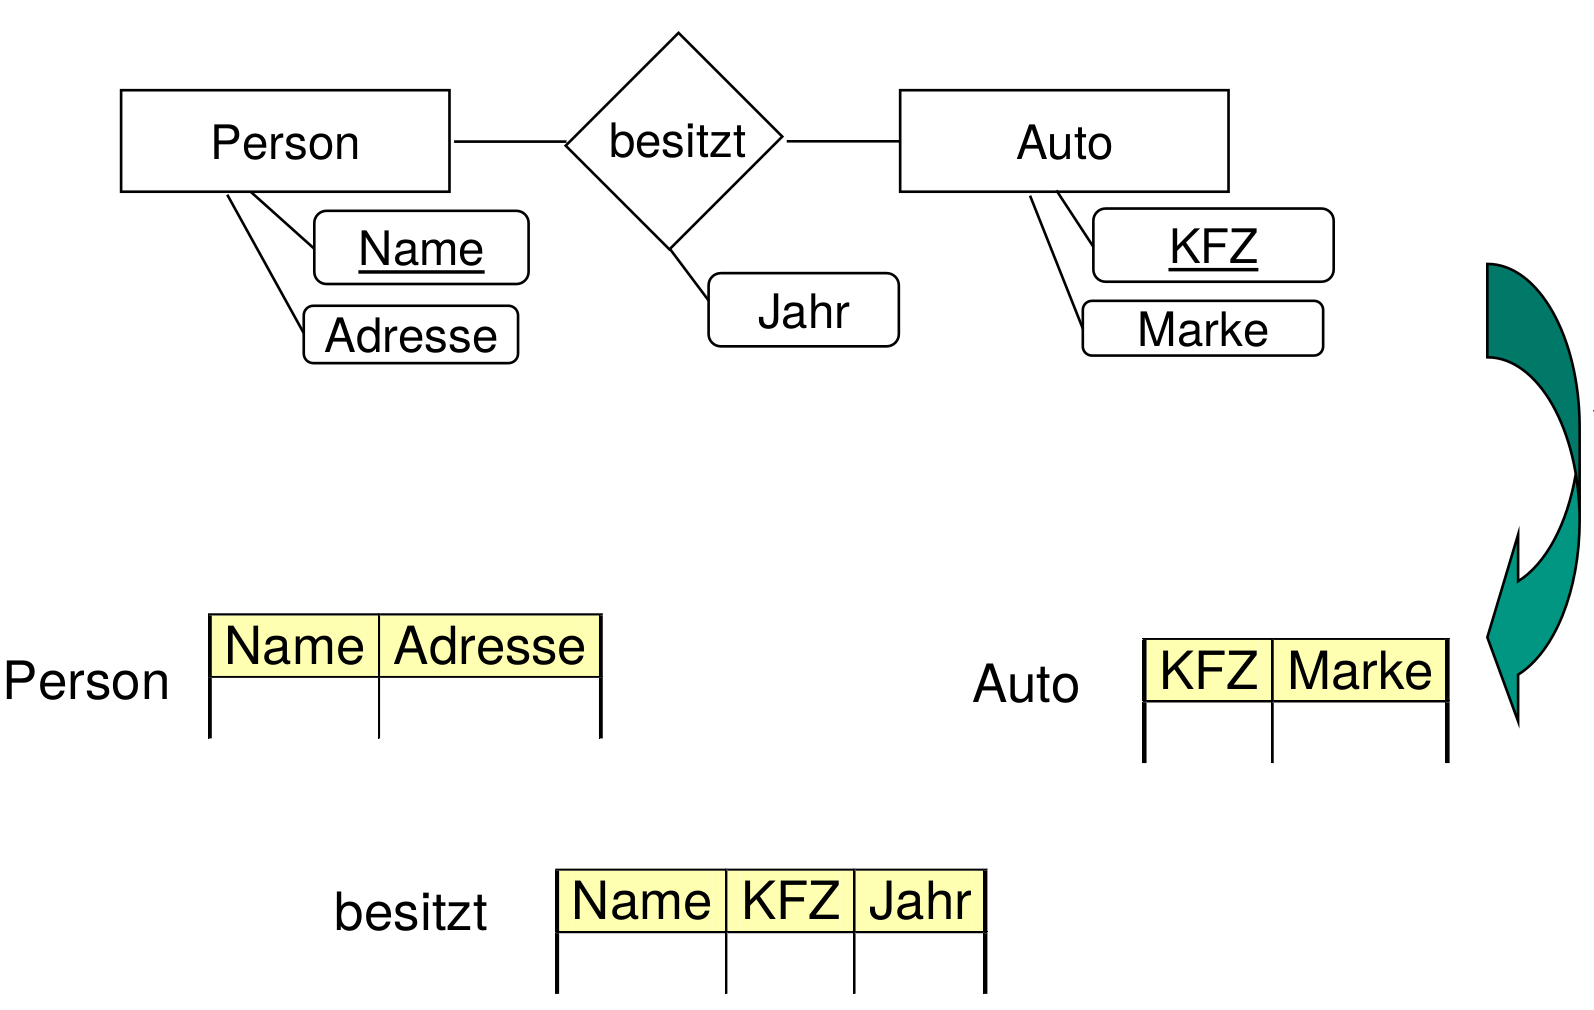
\includegraphics[width=0.33\textwidth]{Abbilden2}\end{figure}

\begin{fragen}
	\begin{enumeration}
		\item Warum gibt es im ER-Modell keine Fremdschlüssel?
		\item Was bedeutet ``kapazitätserhaltende Abbildung''? Geben Sie Beispiele.
		\item Wiedergabe der unterschiedlichen Beziehungsabbildungen (1:1, 1:n, m:n)
		\item In welchen Fällen lässt sich das Schema optimieren? Was bedeutet Optimierung hier?
		\item Wie lassen sich mengenwertige Attribute abbilden?
		\item Warum ist Abbildung der folgenden Konstrukte vom ER-Modell ins Relationenmodell problematisch? Rekursive Beziehungen, Partitionierung, Generalis.
	\end{enumeration}
\end{fragen}